Da stehen wieder ein paar Zeilen. Dieser Text verweist sogar auf das Bild \ref{fig:BildPSP}, welches einen Projektstrukturplan zeigt. Man kann mit \LaTeX auch auf eine Subsection verweisen, wie etwa auf die folgende mit der Nr. \ref{subsec:PSP} verweisen.

\section{Projektstrukturplan}
\label{subsec:PSP}

\begin{figure}
	\centering
	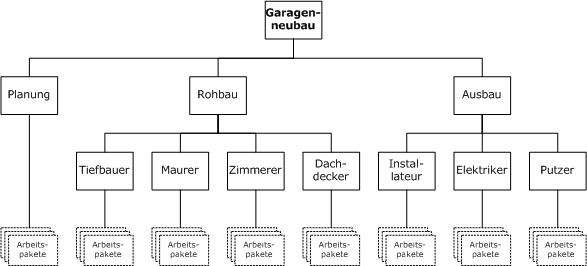
\includegraphics{Bilder/PSP.jpg}
	\caption{Demo-Projektstrukturplan}
	\label{fig:BildPSP}
\end{figure}

\section{Arbeitspakete}
\section{Projektwürdigkeitsanalyse}
\section{Projektdurchführbarkeitsanalyse}
\section{Meilensteinplan}
\section{Tätigkeitsliste - PersonA}

Tabellen einfügen ist in \LaTeX etwas schwieriger. Für das Grundgerüst bieten sich Online-Editoren wie etwa https://latex-editor.pages.dev/table/ an. Dabei ist dann der Tabular-Block zu kopieren.


\begin{table}
\caption{Demotabelle}
\begin{center}
	
\begin{tabular}{ |c|c|c| }
	\hline
	Tätigkeit & Datum & Zeitdauer \\
	\hline
	A         & B     & C         \\
	\hline
	D         & E     & F         \\
	\hline
		D         & E     & F         \\
	\hline
		D         & E     & F         \\
	\hline
		D         & E     & F         \\
	\hline
		D         & E     & F         \\
	\hline
		D         & E     & F         \\
	\hline
		D         & E     & F         \\
	\hline
		D         & E     & F         \\
	\hline
		D         & E     & F         \\
	\hline
\end{tabular}

\end{center}
\end{table}